% Packages
\documentclass[12pt]{article}
\usepackage[margin=2.5cm]{geometry}
\usepackage{lipsum}
\usepackage{titlesec, titletoc}
\usepackage[svgnames, table]{xcolor}
\usepackage{algorithm}
\usepackage{algpseudocode}
\usepackage{mdframed}
\usepackage[T1]{fontenc}
\usepackage{amsmath,amsthm,amsfonts,amssymb,mathtools}
\usepackage[osf]{mathpazo}
\usepackage{enumitem}

% Formating setup
\footskip = 1 cm
\setlength{\parindent}{0pt}
\pdfpxdimen=1in
\parindent = 0pt
\definecolor{myBlue}{RGB}{0, 81, 255}
\titleformat{\section}[block]{\sffamily\large\bfseries}{\thesection}{.5em}{\textcolor{myBlue}
{\titlerule[1.5pt]}\\\sffamily}[\vspace*{-3mm}\textcolor{myBlue}{\titlerule[1.5pt]}]
\titleformat{\subsection}{\large\sffamily\bfseries}{\thesubsection}{0.5em}{\textcolor{Black}}
\newcounter{boxedlistcounter}
\newenvironment{pseudo}{%
  \setcounter{boxedlistcounter}{0}% <-- Add this line to reset the counter
  \mdframed[
    linecolor=black, % color of the border
    linewidth=1.5pt, % thickness of the border
    roundcorner=10pt, % radius of the corners
    innertopmargin=0.6\baselineskip, % space at the top of the box
    innerbottommargin=0.6\baselineskip, % space at the bottom of the box
  ]
  \fontsize{12pt}{14pt}\selectfont % add font size command here
  \mdseries % add font series command here
}{%
  \endmdframed%
}
\newcommand{\I}{\par\stepcounter{boxedlistcounter}\arabic{boxedlistcounter}.\hspace{5pt}}
\newcounter{boxedlistcounter2}
\newenvironment{Proof}{%
  \refstepcounter{boxedlistcounter2}%
  \mdframed[
    linecolor=black, % color of the border
    linewidth=1.5pt, % thickness of the border
    roundcorner=10pt, % radius of the corners
    innertopmargin=\baselineskip, % space at the top of the box
    innerbottommargin=\baselineskip, % space at the bottom of the box
  ]
  \fontsize{12pt}{14pt}\selectfont % add font size command here
  \mdseries % add font series command here
}{%
  \endmdframed%
}
\newcommand{\PI}{\par\textbullet\hspace{5pt}}
\setlist[itemize]{itemsep=1pt}
\newcommand{\NL}{\par\hspace{12.5pt}}
\setlist[itemize]{itemsep=1pt}

% Custom commands
\newcommand{\for}[1]{\textbf{for} #1 \textbf{do}}
\newcommand{\IF}[1]{\textbf{if} #1 \textbf{then}}
\newcommand{\ELIF}[1]{\textbf{else if} #1 \textbf{then}}
\newcommand{\ELSE}{\textbf{else}}
\newcommand{\return}[1]{\textbf{return} #1}
\newcommand{\assign}{ $\leftarrow$ }
\newcommand{\DEF}[2]{\textbf{def} #1(#2):}
\newcommand{\1}{\space \quad}
\newcommand{\2}{\quad \quad \quad}
\newcommand{\3}{\quad \quad \quad \quad \space}
\newcommand{\4}{\quad \quad \quad \quad \quad \quad}
\newcommand{\comment}[1]{\hfill \textit{\# #1}}

% Document start ------------------------------------------------------------------------------------
\begin{document}

% Section 1  ----------------------------------------------------------------------------------------
\section{Map ADT}
\begin{itemize}
  \item get(k): if the map M has an entry with key k, return its associated value.
  \item put(k, v): if key k is not in M, then insert (k, v) into the map M; else, replace the existing value associated to k with v.
  \item remove(k): if the map M has an entry with key k, remove it.
  \item size(), isEmpty()
  \item entrySet(): return an iterable collection of the entries in M.
  \item values(): return an iterable collection of the values in M.
  \item keySet(): return an iterable collection of the keys in M.
\end{itemize}

\subsection{Sorted map ADT (extra methods)}
\begin{itemize}
  \item firstEntry() returns the entry with the smallest key; if map is empty, returns null.
  \item lastEntry() returns the entry with the largest key; if map is empty, returns null.
  \item ceilingEntry(k) returns the entry with the least key that is greater than or equal to k (or null, if no such entry exists).
  \item floorEntry(k) returns the entry with the greatest key that is less than or equal to k (or null, if no such entry exists).
  \item lowerEntry(k) returns the entry with the greatest key that is strictly less than k (or null, if no such entry exists).
  \item higherEntry(k) returns the entry with least key that is strictly greater than k (or null, if no such entry exists).
  \item subMap(k1,k2) returns an iteration of all the entries with key greater than or equal to k1 and strictly less than k2.
\end{itemize}

\subsection{List-Based (unsorted) Map}
We can implement a map using an unsorted list of key-item pairs
To do a get and put we may have to traverse the whole list, so
those operations take O(n) time.
Only feasible if map is very small or if we put things at the end
and do not need to perform many gets (i.e., system log) 

\subsection{Tree-Based (sorted) Map}
We can implement a sorted map using an AVL tree, where each
node stores a key-item pair
To do a get or a put we search for the key in the tree, so these
operations take O(h) time, which can be O(log n) if the tree is
balanced.
Only feasible if there is a total ordering on the keys

% Section 2  ----------------------------------------------------------------------------------------
\section{Hash Functions and Hash Tables}

\subsection{Simple Map Implementation with restricted keys}
Maps support the abstraction of using keys as addresses to get items. Consider a restricted setting in which a 
map with n items with keys in a range from 0 to N-1, for some N >= n. This can be implemented through an array of size
N. The key can be indexed such that entries can be located directly. O(1) operations (get, put, remove).

\vspace{10pt}
The drawback is that usually N >> n, e.g. StudentID is 9 digits, so a Map with StudentID key can be stored in array of 1,000,000,000 entries
(way more than the number of students). This results in bad space utilization.

\subsection{Hash Functions and Hash Tables}
To get around these issues, we use a hash function h to map keys to corresponding indices in an array A.
\begin{itemize}
  \item h must be a mathematical function (always gives same answer for any particular x) and fairly efficient to compute.
  \item Example: h(x) = x mod N is a hash function for integer keys.
  \item The integer h(x) is called the hash value of key x.
\end{itemize}
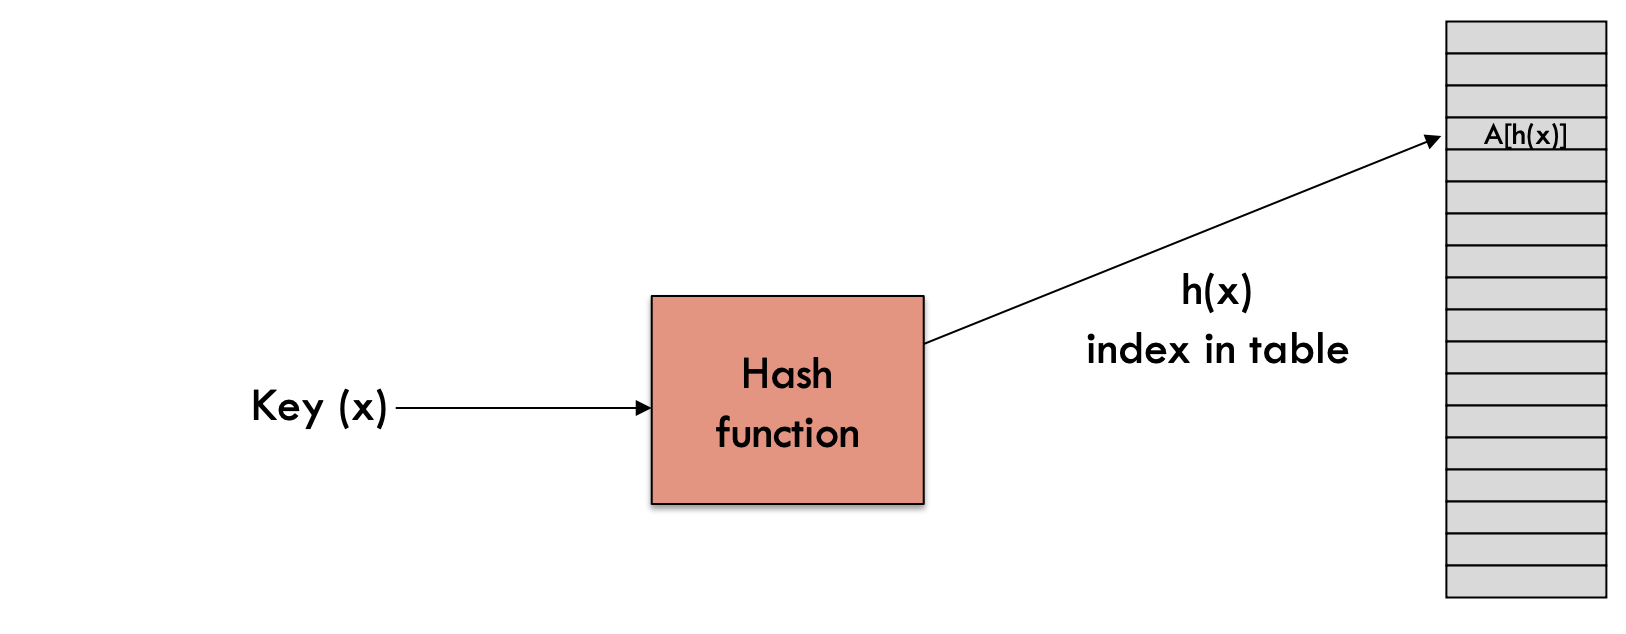
\includegraphics[width=\textwidth]{image12.png}

\textbf{A hash function h is usually the composition of two functions:}
\begin{itemize}
  \item Hash code: h1: Keys to integers (If the keys are not already integers).
  \item Compression function: h2: Integers to [0, N-1].
\end{itemize}
As such, h(x) = h2(h1(x)). The goal of the hash function is to “disperse” the keys in an apparently random way. In general, we want to 
avoid having many items being hashed to the same location.

% Section 3  ----------------------------------------------------------------------------------------
\section{General Approaches}
There are two general approaches that one can take when designing a hash function:

\begin{enumerate}
\item \textbf{View the key k as a tuple of integers}: In this approach, the key is seen as a tuple of integers $(x_1, x_2, \ldots, x_d)$ with each integer being in the range $[0, M-1]$ for some $M$.
\item \textbf{View the key k as a large nonnegative integer}: In this approach, the key is seen as a large nonnegative integer that may have arbitrary length.
\end{enumerate}

\subsection{Summing Components Approach}
The summing components approach is used for keys of the form $k = (x_1, x_2, \ldots, x_d)$.
\begin{itemize}
\item $h(k) = \sum\limits_{i=1}^{d} x_i$
\item $h(k) = (\sum\limits_{i=1}^{d} x_i) \text{ mod } p$, where $p$ is a prime number
\item $h(k) = \sum\limits_{i=1}^{d} x_i \cdot a^{d-i}$, where $a$ is some + integer chosen empirically to avoid collisions.
\end{itemize}
The first two options may cause problems because the hash codes are invariant under permutations of the key tuple. For example, "mate", "meat", "tame", and "team" all map to the same code. The third option solves this problem by making the hash code dependent on the order of the tuple.

\subsection{Modular Division Approach}
The modular division approach is used for keys that are positive integers.
\begin{itemize}
\item $h(k) = k \text{ mod } N$, where $N$ is some prime number.
\end{itemize}
If the keys are randomly and uniformly distributed in $[0, M]$ where $M \gg N$, then the probability that two keys collide is $1/N$. However, keys are usually not randomly distributed, so this approach may not work well in practice.
\subsection{Universal Hash Functions}
A universal hash function is a type of hash function that is designed to produce a relatively uniform distribution of hash values for different input data, regardless of the specific characteristics of the input. To achieve this, a universal hash function uses randomization or other techniques to make the mapping between inputs and hash values unpredictable and independent of the input data.
Universal hash functions are commonly used in various applications that require efficient and secure data hashing, such as cryptography, data compression, and data indexing, among others.

\subsection{Random Linear Hash Functions}
Used on keys k that are positive integers.
\begin{itemize}
\item $h(k) = ((a k + b) \text{ mod } p) \text{ mod } N$
\end{itemize}
Where $p$ is a prime number, and $a$ and $b$ are chosen uniformly at random from the interval $[1, p-1]$ with $a \neq 0$.
The random choice of $a$ and $b$ ensures that the mapping between the keys and hash codes is unpredictable and independent of the specific characteristics of the input data. This makes the hash function resistant to certain types of attacks, such as those based on knowledge of the input data.
One useful property of Random Linear Hash Functions is that if the keys are in the range $[0, M]$ and $p > M$, then the probability that two keys collide is $1/N$. 

% Section 4  ----------------------------------------------------------------------------------------
\section{Collision Handling}
\subsection{Seperate Chaining}
Let each cell in the table point to a linked list holding the entries that map there
Get, put, and remove operations are delegated to the appropriate list, where put
needs to search through the list to replace the existing value of
the key, if present Separate chaining is simple, but requires additional memory
outside the table.
\begin{pseudo}
  \I \DEF{get}{k}
  \I \1 \return{A[h(k)].get(k)}
\end{pseudo}
\begin{pseudo}
  \I \DEF{put}{k,v}
  \I \1 \return{A[h(k)].put(k,v)}
\end{pseudo}
\begin{pseudo}
  \I \DEF{remove}{k}
  \I \1 \return{A[h(k)].remove(k)}
\end{pseudo}
Assume that our hash function maps $n$ keys to independent uniform random values in the range $[0, N-1]$. Let $X$ be a random variable representing the number of items that map to a bucket in the array $A$. Then, $E(X) = n/N$, where the parameter $n/N$ is called the load factor of the hash table, usually denoted as $a$.
The expected time for hash table operations is $O(1+a)$ when collisions are handled with separate chaining. However, the worst-case time is $O(n)$, which happens when all the items collide into a single chain.

\subsection{Linear Probing}
Linear Probing is a technique for handling collisions in a hash table by placing the colliding item in the next available cell (circularly). In other words, if the initial cell is already occupied, the algorithm checks the next cell, and so on until it finds an empty cell.
Each cell inspected during the search for an empty cell is referred to as a probe. Colliding items can end up lumped together, causing future collisions to result in a longer sequence of probes.
Linear Probing can be efficient when the load factor of the table is low, but as the table becomes more crowded, the likelihood of long sequences of probes and poor performance increases. 
\begin{pseudo}
  \I \DEF{get}{k}
  \I \1 i = h(k)
  \I \1 p \assign $0$
  \I \1 repeat
  \I \2 c \assign A[i]
  \I \2 \IF{c = null}
  \I \3 \return{null}
  \I \2 \ELIF{c.key = k}
  \I \3 \return{c.value}
  \I \2 \ELSE
  \I \3 i = (i+1) mod N
  \I \3 p = p + 1
  \I \1 until p = N
  \I \1 \return{null}
\end{pseudo}
\textbf{Updates with Linear Probing}\\
To handle insertions and deletions, we introduce a special object,
called DEFUNCT, which replaces deleted elements, to tell them
apart from empty cells
\begin{itemize}
  \item get(k): must pass over cells with DEFUNCT and keep probing until the element is found, or until reaching an empty cell.
  \item put(k,v): search for the entry as in get(k), but we also remember the index j of the first cell we find that has DEFUNCT or empty. If we find key k, we replace the value there with v and return the previous value. If we don’t find k, we store (k, v) in cell with index j Throw exception if table is full.
  \item remove(k): search for the entry as in get(k). If found, replace it with the special item DEFUNCT and return element v
\end{itemize}
In the worst case, get, put, and remove take O(n) time.
Fact: Assuming hash values are uniformly randomly distributed,
expected number of probes for each get and put is 1/(1-a)
where a = n/N is the load factor of the hash table.
Thus, if the load factor is a constant < 1 then the expected running
time for the get and put operations is O(1).

\subsection{Cuckoo hashing}
Main problem with the methods we’ve seen so far is that operations
take O(n) time in the worst-case.
Cuckoo hashing achieves worst-case O(1) time for lookups and
removals, and expected O(1) time for insertions.
In practice Cuckoo hashing is 20-30\% slower than linear probing but
is still often used due to its worst case guarantees on lookups.

\vspace{10pt}

\textbf{The Power of Two Choices}

\vspace{10pt}
The Power of Two Choices is a technique for handling collisions in a hash table that uses two hash tables, $T1$ and $T2$, each of size $N$, and two hash functions, $h1$ and $h2$, for $T1$ and $T2$ respectively.

\vspace{10pt}
For an item with key $k$, there are only two possible places where we are allowed to store the item: $T1[h1(k)]$ or $T2[h2(k)]$. This restriction simplifies lookup dramatically, while still allowing worst-case $O(1)$ running time for get and remove operations.

\vspace{10pt}
The Power of Two Choices works by randomly selecting which of the two hash tables to use for each item, based on the hash codes generated by the two hash functions. By using two hash tables and two hash functions, the technique reduces the likelihood of collisions and spreads the items more evenly across the tables, improving performance.





\end{document}

